
\section{\trHypersurface{}的\trCharacteristicLineBundle}
\label{sec:characteristic-line-bundle}

\hzsync{theorem}{2}
\hzsync{proposition}{3}
\hzsync{corollary}{2}

在一条给定的\trEnergySurface{} $S$ 上寻找\trHamiltonianVectorField{}的%
\trPeriodicOrbit{}这件事，与表示 $S$ 的那个\trHamiltonianFunction{}的选取无关：%
它只依赖于\trSubmanifold{} $S$ 与\trSymplecticStructure{} $\omega$。的确，%
正如第 1 章中所解释的，这个动力学问题可以用几何方式来描述。我们考察一个%
\trCodimension{}为 1 的\trSubmanifold{} $S\subset M$，即\trSymplecticManifold{}%
$(M,\omega)$ 的一个\trHypersurface。这时，\trSymplecticStructure{} $\omega$%
与 $S$ 便按下述方式确定了一个特殊的\trLineBundle{} $\mathcal{L}_{S}\subset TS$。%
若 $x\in S$，则 \trTwoForm{} $\omega$ 在奇数维子空间 $T_{x}S\subset T_{x}M$ 上的%
限制必是\trDegenerate{}的。这个限制的\trKernel{}维数为 1，这是因为 $\omega$%
在 $T_{x}M$ 上是\trNondegenerate{}的，从而它定义了一个\trLineBundle{}%
$\mathcal{L}_{S}\subset TS$：\footnote{原书印作「$(x,\xi)\in T_{x}S$」，有序对不能属于固定纤维 $T_{x}S$，应为全空间 $TS$（$x$ 取 $(x,\xi)$ 的基点），此处径改。——译者注}
\[
\mathcal{L}_{S}\ =\ \Bigl\{(x,\xi)\in TS\ \Bigm|\ \omega_{x}(\xi,\eta)=0\
\ \text{对一切}\ \eta\in T_{x}S\Bigr\}\ .
\]
这个\trLineBundle{}给出了以 $S$ 为一个\trRegular\trEnergySurface{}的每个%
\trHamiltonianVectorField{}的方向。

\begin{proposition}\label{prop:xh-in-characteristic}
设\trSmooth{}函数 $H$ 把 $S$ 表示成 $S=\bigl\{x\ \bigm|\ H(x)=\text{常数}\bigr\}$，%
并且在 $S$ 上满足 $dH\neq0$，那么
\[
X_{H}(x)\in\mathcal{L}_{S}(x)\qquad\text{对一切}\ x\in S\ .
\]
\end{proposition}

\begin{proof}
由于\trTangentSpace{}由%
$T_{x}S=\bigl\{\xi\in T_{x}M\ \bigm|\ dH(x)\xi=0\bigr\}$ 给出，我们便有%
$\omega\bigl(X_{H}(x),\xi\bigr)=-dH(x)\xi=0$，对一切 $\xi\in T_{x}S$。
\end{proof}

\textbf{记号。}\quad 丛 $\mathcal{L}_{S}$ 称为\trHypersurface{} $S$ 的%
\trCharacteristicLineBundle。$S$ 的一条\trClosedCharacteristic，或 $S$ 的一条%
\trPeriodic\trHamiltonian\trOrbit，是指一条\trEmbedding{}的\trCircle{}%
$P\subset S$，它满足
\[
TP\ =\ \mathcal{L}_{S}\big|_{P}.
\]
在下文中，我们将把 $S$ 的\trClosedCharacteristic{}之集记作
\[
\mathcal{P}(S).
\]
它与以 $S$ 为\trRegular\trEnergySurface{}的每个\trHamiltonianVectorField{}%
$X_{H}$ 在 $S$ 上的未参数化\trPeriodicSolution{}之集相一致。

现在假设 $\mathcal{L}_{S}\to S$ 是\trOrientable{}的，即该丛拥有一个无处为零的%
\trSection。我们将证明：在 $S$ 的一个\trNeighborhood{}上存在着\trHamiltonianFunction{}%
$H:U\to\R$，它把 $S=H^{-1}(0)$ 表示为一个\trRegular\trEnergySurface。我们要%
利用 $M$ 上一个与 $\omega$ \trCompatible{}的\trAlmostComplexStructure，即一个%
满足 $J^{2}=-\mathbf{1}$ 与
\[
\omega(x)\Bigl(\xi,J(x)\eta\Bigr)\ =\ g(x)\,(\xi,\eta)
\]
的\trLinear\trMapping{} $J(x)\in\mathcal{L}(T_{x}M)$（$x\in M$）的\trSmooth{}族，%
其中等式对一切 $\xi$, $\eta\in T_{x}M$ 成立，而 $g$ 是一个\trRiemann{}度量。

若 $N_{S}\to S$ 是 $S$ 的\textbf{\trNormalBundle{}}（normal bundle），其在 $x\in S$ 处的%
\trFiber{}定义为
\[
N_{S}(x)\ =\ \Bigl\{\eta\in T_{x}M\ \Bigm|\ g(x)(\eta,\xi)=0\quad\text{对一切}%
\quad\xi\in T_{x}S\Bigr\},
\]
则我们有丛\trIsomorphism
\[
\mathcal{L}_{S}\to N_{S}\ :\ (x,\xi)\mapsto\Bigl(x,J(x)\xi\Bigr).
\]
这个映射在每根\trFiber{}上确实既是良定义的又是\trInjective{}的：若%
$\omega(\xi,\eta)=0$ 对一切 $\eta\in T_{x}S$ 成立，则%
$g(\eta,J\xi)=\omega\bigl(\eta,J^{2}\xi\bigr)=-\omega(\eta,\xi)=0$。\trNormalBundle{}%
$N_{S}$ 是\trOrientable{}的，因为 $\mathcal{L}_{S}$ 是\trOrientable{}的。于是，$N_{S}$ 与%
$S\times\R$ 作为\trVectorBundle{}是\trIsomorphic。取 $N_{S}$ 的一个无处为%
零的\trSection{} $\sigma$（即 $0\neq\sigma(x)\in N_{S}(x)\subset T_{x}M$），%
我们便能借助\textbf{\trExponentialMap}（exponential map）%
$(x,t)\mapsto\exp_{x}\bigl(t\sigma(x)\bigr)$ 定义\trMapping
\[
\psi\ :\ S\times(-\varepsilon,\varepsilon)\ \to\ U\subset M
\]
当 $S$ 为\trCompact{}且 $\varepsilon$ 充分小时，它是到 $S$ 的一个开\trNeighborhood%
$U$ 上的\trDiffeomorphism。若
\[
F\ :\ S\times(-\varepsilon,\varepsilon)\ \to\ \R
\]
是\trSmooth{}函数 $F(x,t)=t$，则复合 $H=F\circ\psi^{-1}:U\to\R$ 便是所要的那个%
\trHamiltonianFunction；正如所断言的，它满足 $S=H^{-1}(0)$ 与 $dH\neq0$。

\begin{definition}\label{def:parameterized-family}
设 $S$ 为 $(M,\omega)$ 中的一个\trCompact\trHypersurface。以 $S$ 为模型的%
\textbf{\trParameterizedHypersurfaceFamily{}}（parameterized family of hypersurfaces modelled on%
$S$）是一个\trDiffeomorphism
\[
\psi\ :\ S\times I\ \to\ U\subset M,
\]
其中 $I$ 为一个包含 $0$ 的开区间，它映到 $S$ 的一个\trBounded\trNeighborhood{} $U$ 上，且满足
\[
\psi(x,0)\ =\ x\qquad\text{对}\quad x\in S.
\]
\end{definition}

在下文中我们将缩记 $S_{\varepsilon}=\psi\bigl(S\times\{\varepsilon\}\bigr)$，%
并且往后我们常常简单地写 $(S_{\varepsilon})$ 来代替 $\psi$。

我们指出，下列诸陈述是等价的：(i) \trLineBundle{} $\mathcal{L}_{S}\to S$%
是\trOrientable{}的；(ii) \trNormalBundle{} $N_{S}\to S$ 是\trOrientable{}的；(iii) $S$ 是\trOrientable{}的；%
(iv) 存在以 $S$ 为模型的\trParameterizedHypersurfaceFamily{}；(v) 存在定义在 $S$ 的一个开\trNeighborhood%
$U$ 上的\trSmooth{}函数 $H\in C^{\infty}(U,\R)$，它把 $S$ 表示成%
$S=\bigl\{x\in U\ \bigm|\ H(x)=\text{常数}\bigr\}$ 且满足 $dH\neq0$。利用这些%
概念，我们可以把上一节中的\cref{thm:hz-energy-surface}重新表述如下：

\begin{theorem}[\trHofer-\trZehnder]\label{thm:hz-dense-parameterized}
设 $S$ 为 $(M,\omega)$ 中的一个\trCompact\trHypersurface，并设 $(S_{\varepsilon})$%
是以 $S$ 为模型的一个\trParameterizedHypersurfaceFamily{}。若 $c_{0}(U,\omega)<\infty$，则存在一个%
\trDense{}集 $\Sigma\subset I$，使得
\[
\mathcal{P}(S_{\varepsilon})\ \neq\ \emptyset\qquad\text{对}\quad\varepsilon\in\Sigma\ .
\]
\end{theorem}

为了在\trHypersurface{} $S$ 上找到\trClosedCharacteristic——而不只是在其%
近旁——我们现在把所考察的\trHypersurface{}类加以限制。我们假定 $S$ 是一个%
\trCompact\trSymplecticManifold{} $(B,\omega)\subset(M,\omega)$ 的\trBoundary，%
即 $\partial B=S$。

\noindent\begin{minipage}{\linewidth}
\centering
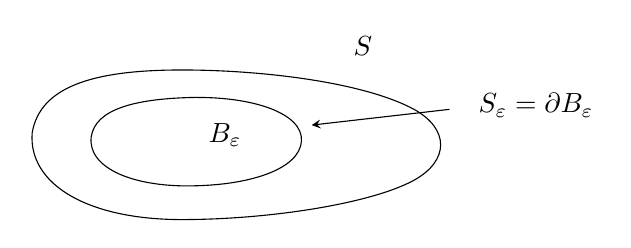
\begin{tikzpicture}[>=stealth,scale=1.0]
  \draw (0.3,0.15) .. controls (0.25,-0.5) and (1.0,-0.95) .. (2.2,-0.95)
        .. controls (3.3,-0.95) and (4.6,-0.75) .. (5.15,-0.45)
        .. controls (5.6,-0.2) and (5.6,0.2) .. (5.15,0.45)
        .. controls (4.5,0.8) and (3.2,0.95) .. (2.2,0.95)
        .. controls (1.1,0.95) and (0.4,0.75) .. (0.3,0.15);
  \node at (4.5,1.25) {$S$};
  \draw (1.05,0.1) .. controls (1.0,-0.3) and (1.6,-0.55) .. (2.4,-0.52)
        .. controls (3.1,-0.5) and (3.7,-0.3) .. (3.72,0.05)
        .. controls (3.74,0.4) and (3.1,0.62) .. (2.3,0.6)
        .. controls (1.6,0.58) and (1.1,0.45) .. (1.05,0.1);
  \node at (2.75,0.12) {$B_{\varepsilon}$};
  \node at (6.7,0.5) {$S_{\varepsilon}=\partial B_{\varepsilon}$};
  \draw[->] (5.6,0.45) -- (3.85,0.25);
\end{tikzpicture}

图 4.4
\end{minipage}

于是，若 $(S_{\varepsilon})$ 是以 $S$ 为模型的一个参数化族，则对%
\trSymplecticManifold{} $B_{\varepsilon}$ 而言有 $S_{\varepsilon}=\partial B_{\varepsilon}$，%
并且我们假定\trParametrization{}的选取使之满足
\[
B_{\varepsilon}\subset B_{\varepsilon'}\qquad\text{若}\quad\varepsilon\leq\varepsilon'.
\]
鉴于\trCapacity{}的\trMonotonicity，我们便有
\[
c_{0}(B_{\varepsilon},\omega)\ \leq\ c_{0}(B_{\varepsilon'},\omega)%
\qquad\text{若}\quad\varepsilon\leq\varepsilon',
\]
从而函数
\[
C(\varepsilon)\ :=\ c_{0}(B_{\varepsilon},\omega)
\]
是单调递增的。

\begin{definition}\label{def:c0-lipschitz-type}
\trHypersurface{} $S_{\varepsilon^{*}}$ 称为\textbf{$c_{0}$-\trLipschitz{}型}%
（$c_{0}$-Lipschitz type）的，如果存在正常数 $L$ 与 $\mu$，使得
\[
C(\varepsilon)\ \leq\ C(\varepsilon^{*})\,+\,L\,(\varepsilon-\varepsilon^{*})
\]
对区间 $\varepsilon^{*}\leq\varepsilon\leq\varepsilon^{*}+\mu$ 中的每个%
$\varepsilon$ 都成立。
\end{definition}

利用 $c_{0}$ 的\trMonotonicity，容易验证这个定义不依赖于以%
$S_{\varepsilon^{*}}$ 为模型的族 $S_{\varepsilon}$ 的选取。我们用一个例子来%
阐释这个概念。设 $S=\partial B$ 是\trCompact{}\trManifold{} $B$ 的\trBoundary，并假定在%
$B$ 的一个\trNeighborhood{}中存在\trVectorField{} $X$ 满足
\begin{align*}
\text{(i)}\qquad & L_{X}\omega\ =\ \omega\\
\text{(ii)}\qquad & X(x)\notin T_{x}S\qquad\text{若}\quad x\in S\ .
\end{align*}

\noindent\begin{minipage}{\linewidth}
\centering
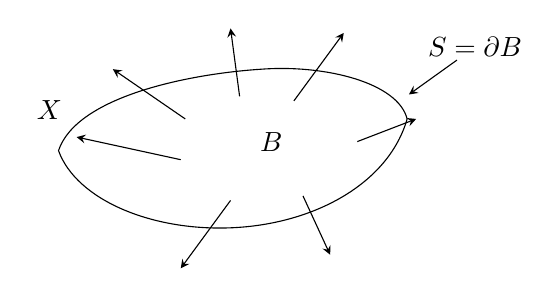
\begin{tikzpicture}[>=stealth,scale=1.15]
  \draw (0.15,0.0) .. controls (0.35,-0.55) and (1.2,-0.9) .. (2.1,-0.85)
        .. controls (3.0,-0.8) and (3.8,-0.35) .. (4.0,0.35)
        .. controls (3.9,0.75) and (3.1,0.95) .. (2.4,0.9)
        .. controls (1.6,0.85) and (0.35,0.6) .. (0.15,0.0);
  \node at (2.5,0.1) {$B$};
  \draw[->] (1.55,0.35) -- (0.75,0.9);%
  \draw[->] (2.15,0.6) -- (2.05,1.35);%
  \draw[->] (2.75,0.55) -- (3.3,1.3);%
  \draw[->] (1.5,-0.1) -- (0.35,0.15);%
  \draw[->] (2.05,-0.55) -- (1.5,-1.3);%
  \draw[->] (2.85,-0.5) -- (3.15,-1.15);%
  \draw[->] (3.45,0.1) -- (4.1,0.35);%
  \node at (0.05,0.45) {$X$};
  \node at (4.75,1.15) {$S=\partial B$};
  \draw[->] (4.55,1.0) -- (4.02,0.62);
\end{tikzpicture}

图 4.5
\end{minipage}

$X$ 的\trFlow{} $\varphi^{t}$ 借助
\[
\psi(x,t)\ =\ \varphi^{t}(x)\ ,\qquad x\in S.
\]
（对充分小的 $|t|$）定义了一个特定的以 $S$ 为模型的\trParameterizedHypersurfaceFamily{}。由%
$L_{X}\omega=\omega$ 可推得 $\bigl(\varphi^{t}\bigr)^{*}\omega=e^{t}\omega$。%
令 $B_{t}:=\varphi^{t}(B)$，映射%
$\varphi^{t}:(B,\omega)\to\bigl(B_{t},e^{-t}\omega\bigr)$ 便是\trSymplectic{}的，%
于是利用 $c_{0}$ 的\trInvariance{}与\trConformality，我们得到%
$e^{-t}c_{0}(B_{t},\omega)=c_{0}\bigl(B_{t},e^{-t}\omega\bigr)=c_{0}(B,\omega)$，%
从而
\[
c_{0}(B_{t},\omega)\ =\ e^{t}\,c_{0}(B,\omega).
\]
函数 $C(t)=c_{0}(B_{t},\omega)$ 在 $t=0$ 处可微，于是我们便验证了 $S$ 是%
$c_{0}$-\trLipschitz{}型的。

\begin{theorem}\label{thm:lipschitz-boundary-closed}
设 $c_{0}(M,\omega)<\infty$。若\trCompact\trHypersurface{} $S\subset M$ 是某个%
\trSymplecticManifold{}的\trBoundary，并且此外还是 $c_{0}$-\trLipschitz{}型的，%
那么
\[
\mathcal{P}(S)\ \neq\ \emptyset.
\]
\end{theorem}

\begin{proof}
由假设，我们可找到一个参数化族 $S_{\varepsilon}$，其中 $S=S_{0}$，使得
\begin{equation}\label{eq:c-linear-bound}
C(\varepsilon)\ \leq\ C(0)\,+\,L\cdot\varepsilon
\end{equation}
对 $0\leq\varepsilon\leq\mu$ 成立。对于 $0<\tau<\mu$，我们引入由满足
\begin{align*}
f(s)\ =\ a \qquad & \text{若}\qquad s\leq0\\
f(s)\ =\ b \qquad & \text{若}\qquad s\geq\tfrac{\tau}{2}\\
0<f'(s)\leq c \qquad & \text{若}\qquad 0<s<\tfrac{\tau}{2}
\end{align*}
的诸\trSmooth{}函数 $f:\R\to\bigl(C(0)-\tau L,\infty\bigr)$ 所组成的集合%
$\mathcal{F}_{\tau}$，其中常数 $a$, $b$, $c$ 受如下条件限制：
\begin{align*}
C(0)-L\tau \quad &\leq\quad a \quad\leq\ C(0)\\
C(0)+2L\tau \quad &\leq\quad b \quad\leq\ C(0)+3L\tau\\
c\ &=\ 10L.
\end{align*}
注意 $\mathcal{F}_{\tau}\neq\emptyset$。固定 $\tau$ 并回顾 $c_{0}(B_{0})$ 的%
定义，我们便可找到一个\trAdmissible{}函数 $H\in\mathcal{H}_{a}(B_{0},\omega)$%
满足 $C(0)-L\tau\leq m(H)<C(0)$。然后我们选取一个 $f\in\mathcal{F}_{\tau}$%
使 $a=m(H)$，并如下定义\trHamiltonianFunction{} $F$：
\begin{align*}
F(x)\ =\ H(x) \qquad & \text{若}\qquad x\in B_{0}\\
F(x)\ =\ f(\varepsilon) \qquad & \text{若}\qquad x\in S_{\varepsilon},\
0\leq\varepsilon\leq\tau\\
F(x)\ =\ b \qquad & \text{若}\qquad x\notin\overline{B_{\tau}}.
\end{align*}
显然 $F\in\mathcal{H}\bigl(B_{\tau},\omega\bigr)$，并且由%
\eqref{eq:c-linear-bound} 得
\[
m(F)\ =\ b\ \geq\ C(0)+2L\tau\ >\ C(0)+L\tau\ \geq\ C(\tau).
\]

\noindent\begin{minipage}{\linewidth}
\centering
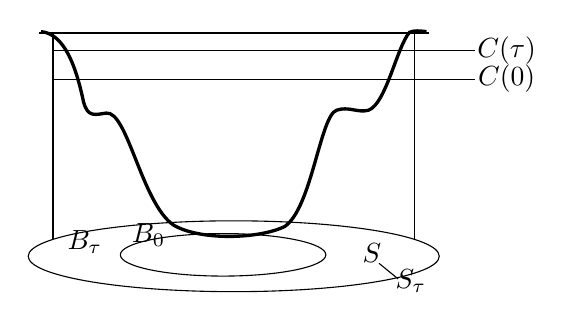
\begin{tikzpicture}[>=stealth,scale=0.9]
  \draw (0.55,0.54) -- (0.55,3.45);%
  \draw (5.65,0.54) -- (5.65,3.45);%
  \draw (0.35,3.45) -- (5.85,3.45);%
  \draw (0.55,3.20) -- (6.5,3.20);
  \draw (0.55,2.80) -- (6.5,2.80);
  \node at (6.95,3.20) {$C(\tau)$};
  \node at (6.95,2.80) {$C(0)$};
  \draw (3.1,0.3) ellipse (2.9 and 0.5);
  \draw (2.95,0.32) ellipse (1.45 and 0.3);
  \node at (1.0,0.5) {$B_{\tau}$};
  \node at (1.9,0.6) {$B_{0}$};
  \node at (5.05,0.35) {$S$};
  \node at (5.6,-0.05) {$S_{\tau}$};
  \draw (5.42,-0.02) -- (5.15,0.2);
  \draw[very thick] (0.38,3.47)
        .. controls (0.72,3.44) and (0.88,2.95) .. (0.98,2.48)
        .. controls (1.04,2.25) and (1.15,2.30) .. (1.30,2.32)
        .. controls (1.60,2.36) and (1.80,1.05) .. (2.25,0.74)
        .. controls (2.62,0.52) and (3.45,0.54) .. (3.82,0.72)
        .. controls (4.20,0.98) and (4.32,2.28) .. (4.55,2.36)
        .. controls (4.72,2.42) and (4.85,2.32) .. (5.00,2.36)
        .. controls (5.25,2.45) and (5.40,3.25) .. (5.58,3.46)
        .. controls (5.65,3.49) and (5.72,3.48) .. (5.82,3.47);
\end{tikzpicture}

图 4.6
\end{minipage}

由于 $m(F)>c_{0}\bigl(B_{\tau},\omega\bigr)=C(\tau)$，我们从\trCapacity{}函数%
$c_{0}$ 的定义推得，\trHamiltonianSystem
\[
\dot{x}\ =\ X_{F}(x)\ ,\qquad x\in B_{\tau}.
\]
拥有一个具周期 $0<T\leq1$ 的非常值\trPeriodicSolution{} $x(t)$。由构造，这个解%
不可能含于 $B_{0}$ 中：因为 $F$ 在 $B_{0}$ 上的限制是一个\trAdmissible{}函数，%
而 $B_{0}$ 在 $X_{F}$ 的\trFlow{}下是\trInvariant{}的，所以解 $x(t)$ 必定含于%
$B_{\tau}\backslash\overline{B_{0}}$ 中。由于该解不是常值的，我们利用 $f$ 的%
性质便可找到 $0<\varepsilon<\tfrac{\tau}{2}$ 中的一个 $\varepsilon$，使得
\[
x(t)\ \subset\ S_{\varepsilon}.
\]
这个论证对每个 $\tau>0$ 都行之有效，于是选取一列 $\tau_{j}\to0$，我们便找到%
序列 $F_{j}$ 与 $\varepsilon_{j}$ 以及 $X_{F_{j}}$ 的相应的\trPeriodicOrbit{}%
序列 $x_{j}(t)$，满足
\[
x_{j}(t)\ \subset\ S_{\varepsilon_{j}}\ ,\qquad\varepsilon_{j}\to0
\]
并且其周期为 $0<T_{j}\leq1$。此外，这些解还满足一些与 $j$ 无关的\trEstimate。%
在
\[
U\ =\ \bigcup_{\varepsilon\in I}S_{\varepsilon}
\]
上，通过令
\[
K(x)\ =\ \varepsilon\qquad\text{若}\quad x\in S_{\varepsilon}.
\]
来定义一个固定的\trHamiltonianFunction{} $K$，它以诸\trHypersurface{}%
$S_{\varepsilon}$ 为其\trRegular\trEnergySurface。若 $x\in S_{\varepsilon}$%
且 $0\leq\varepsilon\leq\mu$，则对每个 $\tau_{j}$ 都有%
$F_{j}(x)=f_{j}\bigl(K(x)\bigr)$，从而%
$X_{F}(x)=f'\bigl(K(x)\bigr)\cdot X_{K}(x)$，此处我们未标明函数 $f$ 与 $F$%
对 $j$ 的依赖。由构造，这些周期函数满足方程
\begin{align*}
\dot{x}_{j}(t)\ &=\ f'\bigl(\varepsilon_{j}\bigr)X_{K}\Bigl(x_{j}(t)\Bigr)\\
x_{j}(0)\ &=\ x_{j}\bigl(T_{j}\bigr)
\end{align*}
并且 $0<T_{j}\leq1$。经重新参数化，函数
\[
y_{j}(t)\ =\ x_{j}\left(\frac{t}{f'(\varepsilon_{j})}\right)
\]
便满足\trHamiltonianEquation
\[
\dot{y}_{j}(t)\ =\ X_{K}(y_{j})\qquad\text{以及}\qquad%
K\Bigl(y_{j}(t)\Bigr)\ =\ \varepsilon_{j}.
\]
现在关键的一步观察是：$y_{j}$ 的周期由%
$f'\bigl(\varepsilon_{j}\bigr)\cdot T_{j}$ 给出，从而（鉴于%
$f'\bigl(\varepsilon_{j}\bigr)\leq10L$\footnote{原书印作「$10M$」，疑为「$10L$」之误（前文已定义 $c=10L$），此处径改。——译者注}）这些周期是有界的。于是，由%
\cref{prop:bounded-periods-limit}
我们得出结论：$X_{K}$ 在\trEnergySurface{} $K(x)=0$（它就是\trHypersurface{}%
$S=S_{0}$）上存在一个\trPeriodicSolution{} $x(t)$，而这个\trPeriodicSolution{}%
便参数化了 $S$ 上所要的那条\trClosedCharacteristic。
\end{proof}

现在回顾一下，上面所定义的函数%
$C(\varepsilon)=c_{0}\bigl(B_{\varepsilon},\omega\bigr)$ 是单调的。于是，由%
\trLebesgue{}的一个定理，它几乎处处可微，从而几乎处处\trLipschitz{}连续；%
由此我们从\cref{thm:lipschitz-boundary-closed}推得

\begin{theorem}\label{thm:almost-every-level}
设\trHypersurface{} $S\subset(M,\omega)$ 是某个\trCompact\trSymplecticManifold{}%
的\trBoundary。若 $(S_{\varepsilon})$（$\varepsilon\in I$）是以 $S$ 为模型的一个%
\trParameterizedHypersurfaceFamily{}，则（$m$ 表示\trLebesgue{}测度）
\[
m\ \Bigl\{\varepsilon\in I\ \Bigm|\ \mathcal{P}(S_{\varepsilon})\neq\emptyset%
\Bigr\}\ =\ m(I),
\]
只要 $c_{0}(M,\omega)<\infty$。
\end{theorem}

一个\trCompact{}且\trConnected{}的\trHypersurface{} $S\subset\R^{2n}$ 把空间%
分离成一个有界的与一个无界的\trConnectedComponent。（的确，每个%
\trCompact\trSmooth\trHypersurface{} $M\subset\R^{m}$ 都是\trOrientable{}的；这一论断%
可由\trJordan-\trBrouwer{}分离定理导出，关于光滑情形的一个简短的微分几何证明，%
我们请读者参阅 E.~\trLima{} [142]。）于是，对于标准\trSymplecticManifold{}%
$\bigl(\R^{2n},\omega_{0}\bigr)$ 中的\trHypersurface{}这一特殊情形，我们便%
得出下述\trhCorollary：

\begin{corollary}\label{cor:standard-almost-all}
对标准\trSymplecticManifold{} $\bigl(\R^{2n},\omega_{0}\bigr)$ 中的每个%
\trCompact\trHypersurface{} $S$ 以及每个以 $S$ 为模型的\trParameterizedHypersurfaceFamily{}%
$(S_{\varepsilon})$（$\varepsilon\in I$），都有
\[
m\ \Bigl\{\varepsilon\in I\ \Bigm|\ \mathcal{P}(S_{\varepsilon})\neq\emptyset%
\Bigr\}\ =\ m(I).
\]
\end{corollary}

这一结果最初由 M.~\trStruwe{}在 [207] 中证明，他巧妙地修改了 H.~\trHofer{}与%
E.~\trZehnder{}在 [123] 中对较弱命题——$\mathcal{P}(S_{\varepsilon})\neq\emptyset$%
对 $I$ 中一个\trDense{}集内的 $\varepsilon$ 成立——所给的证明。作为说明，%
我们取一个\trSmooth{}函数 $H\in C^{\infty}_{c}\bigl(\R^{2n}\bigr)$，即一个具有%
\trCompactSupport{}的函数。这时，\trCritical{}水平之集在 $\R$ 中是\trCompact{}的，%
而且由\trSard{}的\trMeasureZero{}定理它还是\trMeasureZero{}的。于是，对
\[
\min H\ <\ h\ <\ \max H
\]
中的几乎每个 $h$，\trHamiltonianVectorField{} $X_{H}$ 都拥有一个具\trEnergy{}%
$H\bigl(x_{h}(t)\bigr)=h$ 的非常值\trPeriodicSolution{} $x_{h}(t)$。这是%
C.~\trViterbo{} [218] 最近一个针对\trMapping（而非\trVectorField）的结果在局部上的%
类似命题。该结果说：$\bigl(\R^{2n},\omega_{0}\bigr)$ 的一个在\trCompact{}集%
$K\subset\R^{2n}$ 之外为\trIdentityMap{}的\trSymplecticDiffeomorphism{}%
$\varphi$ 拥有无穷多个含于 $K$ 之内的\trPeriodicOrbit。我们应当提到，%
C.~\trViterbo{}还从 $\bigl(\R^{2n},\omega_{0}\bigr)$ 中诸子集的某个%
\trSymplecticInvariant{}的存在性出发导出了他的结果，该不变量与\trCapacity{}%
$c_{0}$ 之间的关系迄今尚不清楚。
